\section{Exercise 3: General Assessment}

\subsection{Finding information with whois}
\subsubsection{What do you learn about SDU's network? In the protocol, note the IP range.}
Running the \texttt{whois} command for the ip address of \href{www.sdu.dk}{www.sdu.dk} gives us a whole bunch of information, such as NetRange, CIDR, the name of the domain organization. The full output would be too long to have in the report as-is, so snippets of the output are showcased as they become relevant. The snippet showing the IP range as well as information about the organization that the site is hosted with can be seen below.

\lstinputlisting[firstline=13, lastline=25]{Outputs/E03/whoisip.txt}

This part of the output tells us that the ip range is 20.33.0.0 to 20.128.255.255 or as denoted by the CIDR format, the following ranges:
\begin{center}
    \begin{tblr}{vlines}
        20.33.0.0/16 & 20.34.0.0/15 & 20.36/0.0/14 & 20.40.0.0/13 & 20.48.0.0/12 & 20.64.0.0/10 & 20.128.0.0/16
    \end{tblr}
\end{center}

\subsubsection{What is the whois information for nextcloud.sdu.dk? What do you observe in comparison to the whois-information you gathered for www.sdu.dk}
Querying \href{https://nextcloud.sdu.dk}{nextcloud.sdu.dk} gives us a bunch of information like when we query the ip address of www.sdu.dk
\vfill
\lstinputlisting[firstline=13, lastline=27]{Outputs/E03/whoisncip.txt}
The output of querying nextcloud.sdu.dk is similar to the output of querying the ip address of sdu.dk without needing to actually query the ip address. Additionally, the ip range of \href{https://nextcloud.sdu.dk}{nextcloud.sdu.dk} is different, being 130.225.128.0 to 130.225.159.255.

\subsection{Question: nmap}
\subsubsection{Nmap scans can be set up to evade firewalls. Which tags would you use for sending packets with specified ip options and spoofing your MAC address?}
In order to send packets with specific ip options, I would use the \texttt{--ip-options} argument as specified in the \href{https://nmap.org/book/man-bypass-firewalls-ids.html}{nmap manual}.

In order to spoof a MAC address, I would use the \texttt{--spoof-mac} argument as specified in the \href{https://nmap.org/book/man-bypass-firewalls-ids.html}{nmap manual}.

\subsection{Comparing the Tools}
\subsubsection{Compare your results from each of the previous activities in each question (e.g, legion, nessus vs gvm). Take notes and discuss overlaps and differences in results, pros and cons, ease of use for each tool.}
The following comparison is made between Legion, Nessus and GVM

Overlaps:
\begin{itemize}
    \item All three tools are used for vulnerability assessment.
    \item Each tool is capable of identifying common vulnerabilities and security flaws in configurations.
    \item All three tools have access to network scanning.
\end{itemize}
Differences:
\begin{itemize}
    \item \textbf{Legion} is open-source and has a bigger focus on network penetration. It has a higher tech literacy requirement.
    \item \textbf{Nessus} is a closed-source product which has a focus on user-friendliness and scanning.
    \item \textbf{GVM}, like Legion, is open-source and has a bigger focus on allowing power users to customize their scans to whatever use case they may have.
\end{itemize}
Pros \& Cons:
\begin{itemize}
    \item \textbf{Legion}
          \begin{itemize}
              \item \textbf{Pros:} Open-source, allows for custom scripting.
              \item \textbf{Cons:} Not very user-friendly and requires prior technical knowledge.
          \end{itemize}
    \item \textbf{Nessus}
          \begin{itemize}
              \item \textbf{Pros:} Very user-friendly.
              \item \textbf{Cons:} Commercial product, not as customizable.
          \end{itemize}
    \item \textbf{GVM}
          \begin{itemize}
              \item \textbf{Pros:} Open-source with always-updating vulnerability database, very customizable.
              \item \textbf{Cons:} Not as intuitive for beginners as Nessus.
          \end{itemize}
\end{itemize}
Ease of Use:
\begin{itemize}
    \item \textbf{Legion:} Technical focus allowing experienced users to get results they need.
    \item \textbf{Nessus:} Very focused on easy usability with a user-friendly interface.
    \item \textbf{GVM:} Complex interface and many options, allowing beginners to easily perform a scan with the flexibility to allow more experienced users to customize.
\end{itemize}

\subsection{Collecting the Assessment Information}
Collecting assessment information for 4 services requires us to first find an ip range that we can scan with GVM. We can find this using the \texttt{ip a} command. The output of this command is shown below.

This gives us two wifi interfaces, however, the only relevant one is the eth0 interface, so that is the one that will be shown. As scanning against both Linux and Windows machines is optional and the ARM-based MacBook that these exercises are performed on seem to have issues with running the Windows Metasploitable image, only the Linux machine will be analyzed for vulnerabilities.

\lstinputlisting[firstline=7]{Outputs/E03/ip\space a.txt}
Under the second internet adapter listing eth0, we can see that the ip range is 10.0.2.4/24. This tells us that our Kali VM is running on 10.0.2.4. This means, that since our VMs are set up in a NAT Network, to perform a full assessment and discover any machines on our network, we must search through 10.0.2.0/24.

\begin{figure}[H]
    \begin{center}
        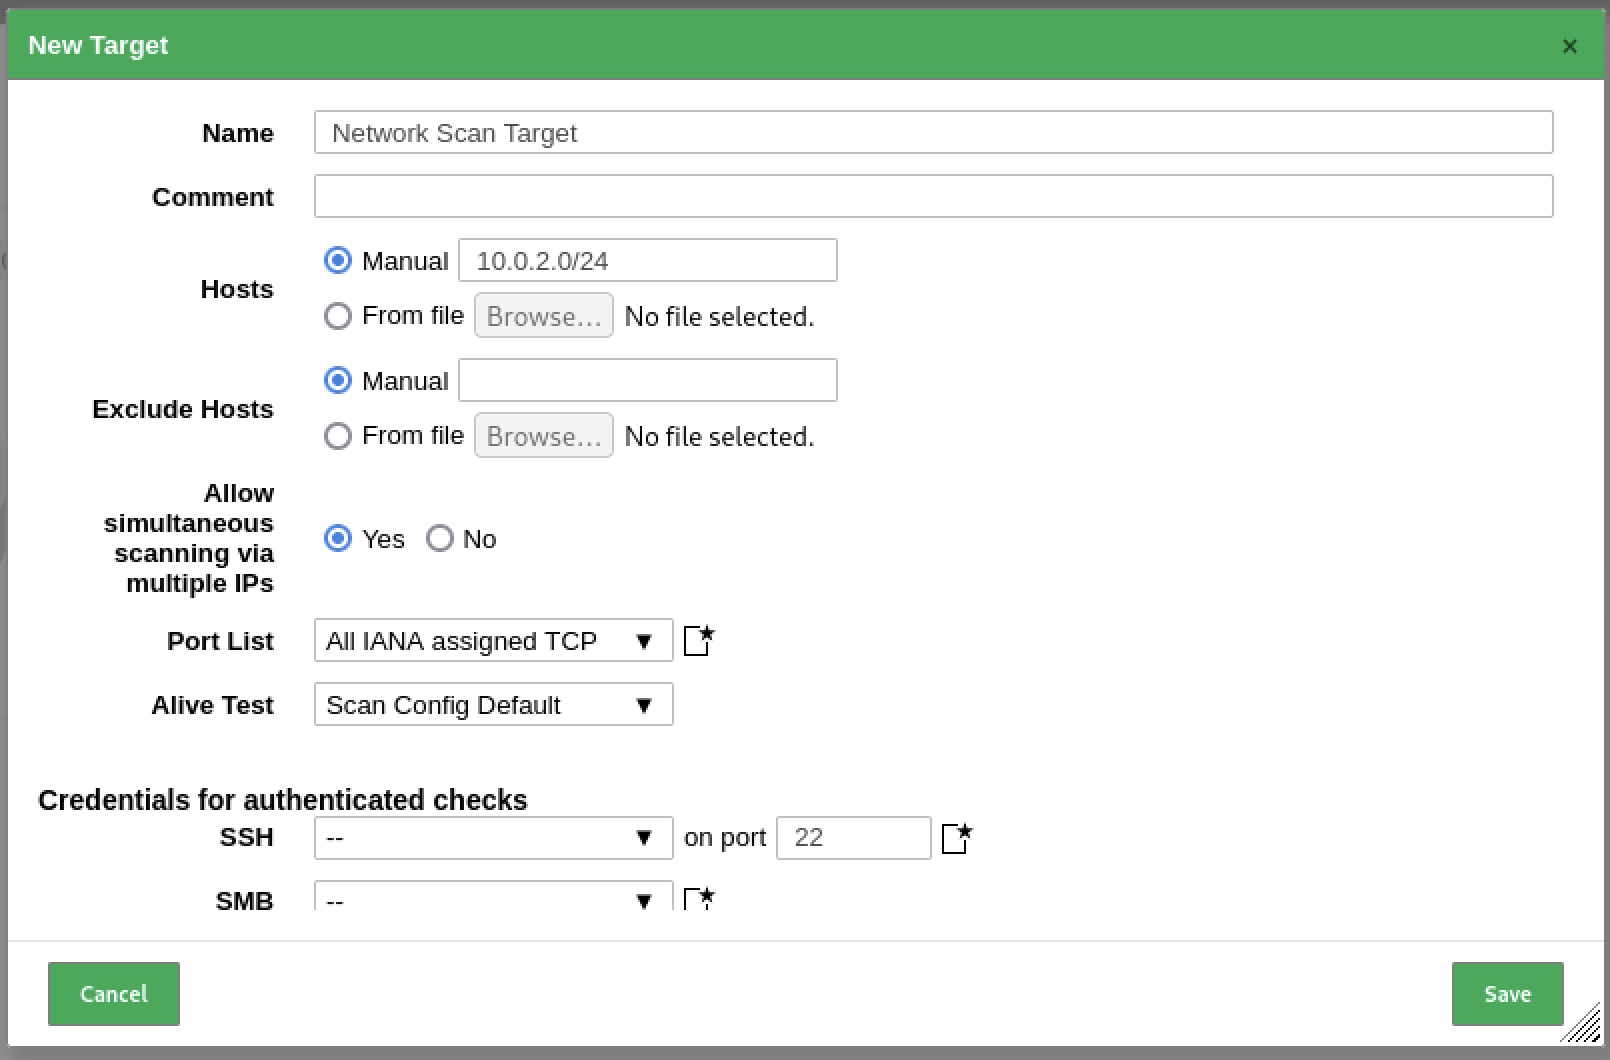
\includegraphics[width=\textwidth]{Outputs/E03/gvm-scan-target.png}
    \end{center}
\end{figure}

To scan a network for machines with vulnerabilities, we need to set up a scan target, which will be the aforementioned 10.0.2.0/24, meaning that we'll scan the network 10.0.2.0 through 10.0.2.255. After setting up this scan target, we can define a scan task with the scan target that we just created, which will generate a report for us on all available services, vulnerabilities, their CVE, what machine they're located on and more.

\begin{figure}[H]
    \begin{center}
        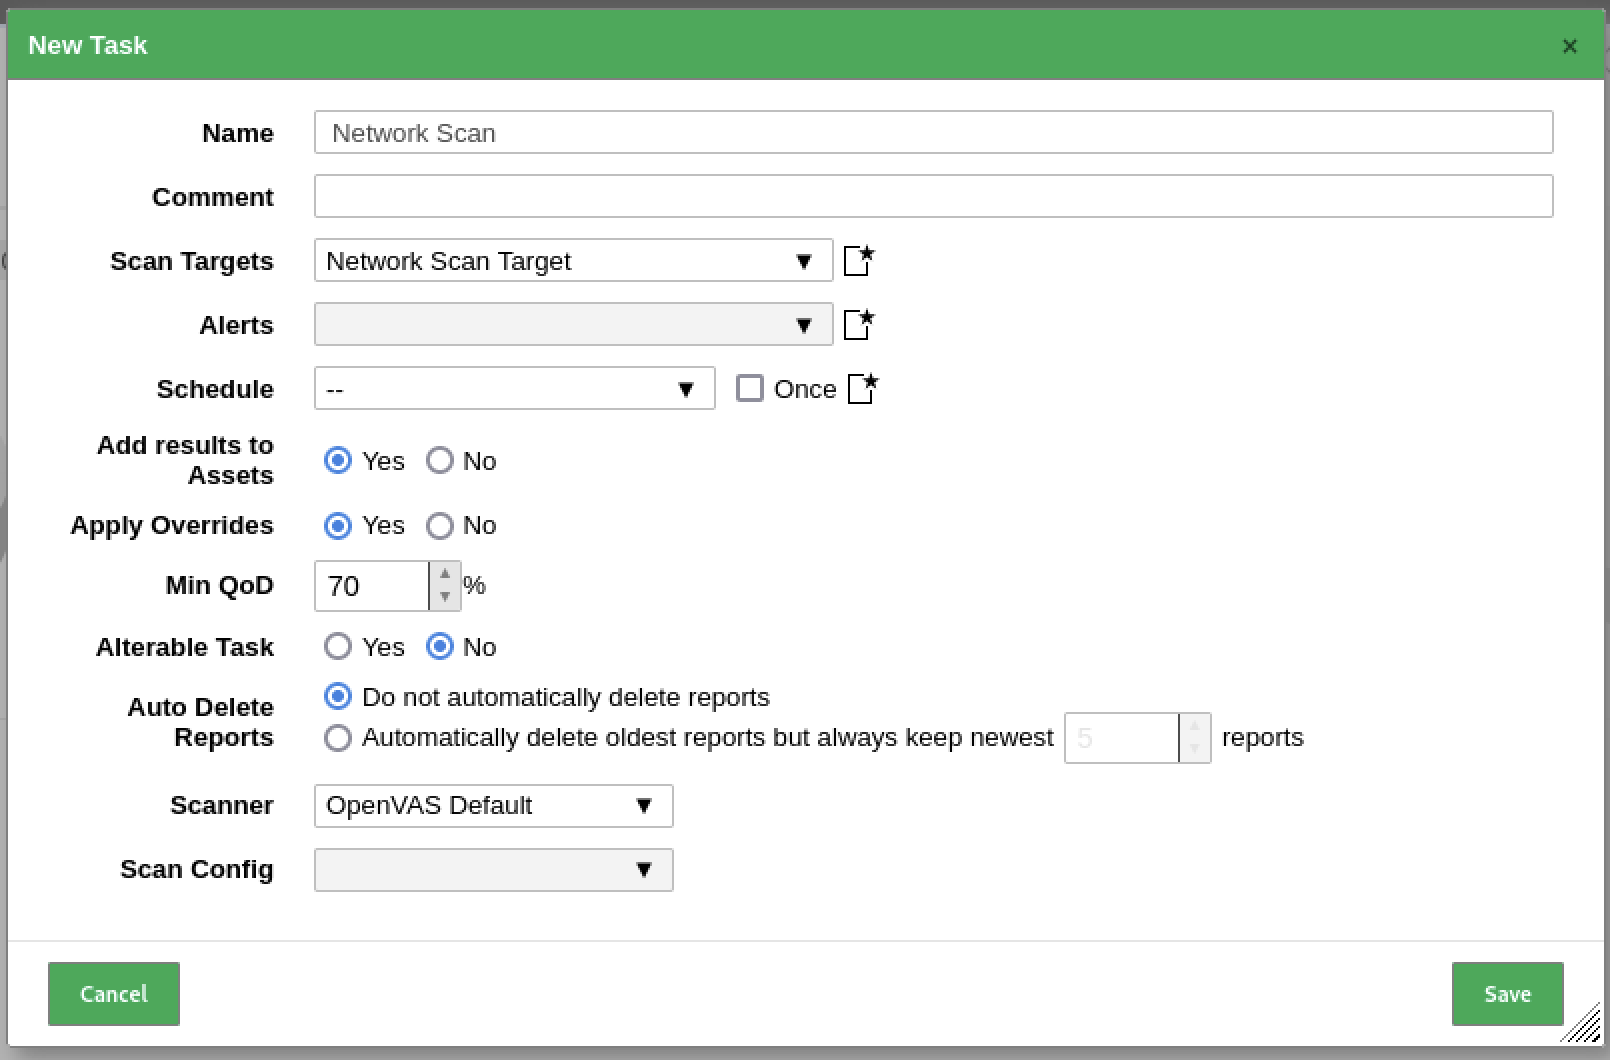
\includegraphics[width=\textwidth]{Outputs/E03/gvm-task.png}
    \end{center}
\end{figure}
\subsubsection{Service, port number and version number}
Based on the previous GVM scan report, four vulnerable services located on the Linux machine were selected for analysis.

The four services that were selected to be analyzed are:
\begin{itemize}
    \item FTP, 21 ProFTPD 1.3.5
          \begin{itemize}
              \item \textbf{Vulnerability:} ProFTPD allows for unauthenticated copying of files, which could potentially result in remote code execution.
              \item \textbf{Severity:} It has a very high severity, as remote code execution is one of the worst exploits to have available on a machine.
              \item \textbf{Source:} \href{https://cve.mitre.org/cgi-bin/cvename.cgi?name=CVE-2015-3306}{CVE-2015-3306}
          \end{itemize}
    \item SSH, 22, OpenSSH 6.6.1p1 Ubuntu 2ubuntu2.13 (Ubuntu Linux; protocol 2.0)
          \begin{itemize}
              \item \textbf{Vulnerability:} OpenSSH allows signing in to a minikube container with default credentials, allowing anyone to bypass authentication.
              \item \textbf{Severity:} The severity is very high, as allowing users to bypass any part of the security of an SSH connection, could result in further unauthorized access and potentially remote access to a full machine's shell.
              \item \textbf{Source:} \href{https://cve.mitre.org/cgi-bin/cvename.cgi?name=CVE-2023-1944}{CVE-2023-1944}
          \end{itemize}
    \item HTTP, 80, Apache httpd 2.4.7
          \begin{itemize}
              \item \textbf{Vulnerability:} Drupal allows remote code execution through the drupal\_coder module, which is accessible through the open directory listing in Apache httpd.
              \item \textbf{Severity:} This is very high severity for the same reason as the vulnerability of ProFTPD. Remote code execution is very dangerous.
              \item \textbf{Source:} \href{https://www.drupal.org/node/2765575}{https://www.drupal.org/node/2765575}
          \end{itemize}
    \item IPP, 631, CUPS 1.7
          \begin{itemize}
              \item \textbf{Vulnerability:} The service is using outdated versions of TLS, potentially making decryption of connections possible, no longer making it safe to send sensitive data over said connection.
              \item \textbf{Severity:} The severity isn't too high, as sensitive data isn't necessarily being sent over the connection.
              \item \textbf{source:} \href{https://cve.mitre.org/cgi-bin/cvename.cgi?name=CVE-2011-3389}{CVE-2011-3389}
          \end{itemize}
\end{itemize}

\subsection{Completing the Assessment}
\subsubsection{Final report}
Based on the information found in the previous assessment analysis via the detailed GVM report that was generated, it is clear that the Linux machine has several very large security holes with high severity. Many of these vulnerabilities allow for remote code execution, reverse shells and equally dangeorous exploits, which can leave a machine fully open to further exploitation. Therefore, in order to avoid these issues in the future, the recommendation is to immediately take the system offline, update any packages to at least their newest secure version.

Additionally, after performing these upgrades, it is recommended that tools such as GVM is used to continuously and regularly create reports to ensure that all holes have been patched and that new exploits have not been found that put the system in danger once again.